\section{First Program: Hello World} \label{first}

This section introduces the first C program, it is commonly called \textit{HelloWorld}. It simply prints out a "Hello World" string to a terminal console. This simple program actively tests out both the C compiler and the host Operating System.\\ 

Rather than wait let's dive right into the code.\\

\begin{lstlisting}[language=C,showstringspaces=false,caption={File hellow1.c, C Hello World example},captionpos=b,label=helloworld]
 1 #include <stdio.h>
 2 
 3 int main(void)
 4 {
 5 printf("Hello World\n");
 6
 7 return 0;
 8 }
\end{lstlisting}

\parskip = \baselineskip

The entire program is shown in listing \ref{helloworld}. The first line or line:1 contains \textit{\#include \textless stdio.h\textgreater}. The \textit{\#include} directive is part of the preprocessor phase of the compilation process. We will discuss the preprocessor phase in more detail later. It is a powerful feature which can be abused with overuse. This particular directive brings in the library header file called \textit{stdio.h} (called Standard IO). \textit{stdio.h} \index{stdio.h} library is part of the ISO C Standard. It contains a number of useful functions. One particular useful function, \textit{printf(...)}, is used by the \textit{HelloWorld} example.

 \textit{printf(...)} function \index{printf(...)} on line:5 sends the \textit{"Hello World\escape{n}"} string to the console. The output text is the string enclosed by "...". The string also includes \escape{n} located at the end of the text. \escape{n} represents a newline and instructs the Operating System to print out all the characters in the output buffer.

Line:3 has \textit{int main(void)} \index{main(...)}. This provides three useful pieces of information, namely the function call name, input parameters to the function and the return output type of the function. The name in this example is \textit{main}. The input is \textit{(void)} and finally the output is \textit{int}. The actual function name \textit{main} is special. It is both a unique name for a function and it is the name given for the entry point of every C program. It is the first user code executed in a program.

This means that every C program has to include a \textit{main(...)} function. Missing this function will result in an error being raised. Prior to \textit{main(...)} being called, initialization code is executed. This code sets up internal variables, the C runtime stack and finally invokes \textit{main(...)}. If \textit{main(...)} is not present an \textit{unresolved function call error} is raised during compilation i.e. the standard C entry point is absent.

For deeply embedded systems or bare metal embedded systems, the \textit{main(...)} function can be optional. This is because embedded engineers quite often want to control the initialization code e.g. configure physical pins, setup the internal clocks, etc.. This means that any arbitrary C function can be used as the entry point. 

\textit{(void)} input parameters on line:3 means that the function requires no input parameters. Note, \textit{main(...)} can have special parameters called \textit{argv} and \textit{argc} as input parameters. These parameters allow command line arguments to be passed into a program. If you are interested in this specific feature it is recommended that you explore the \textit{main(...)} parameters options in more detail.

The \textit{int} output means the function \textit{main(...)} return-type is a signed integer value.

Line:4 \textit{\{} open curly bracket is used to symbolize the start of the function body. There is alway a reciprocal close curly bracket \textit{\}} to end the function body. This is different to languages such as Python which use a different method to identify the start and end of function bodies.

Lastly line:7 contains \textit{return 0;}. \index{return} This returns a value to the callee routine outside the function. In this case it is the end of the program and the value 0 is passed to the host Operating System. Non 0 values symbolize an error has occurred during program execution.

\begin{figure}[H]
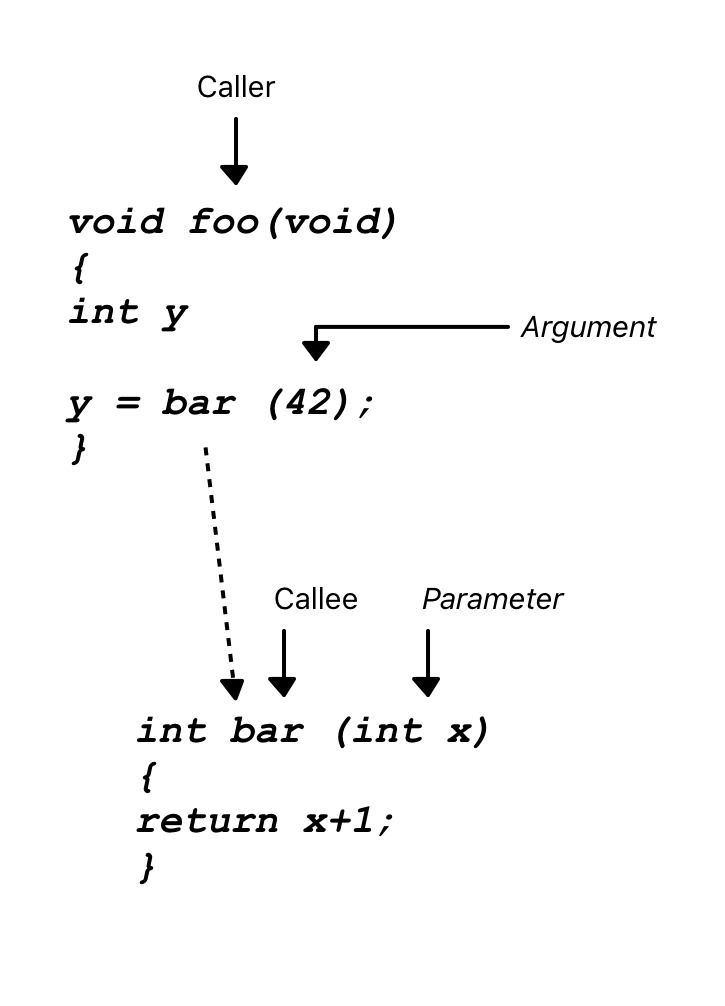
\includegraphics[width=0.4\textwidth]{callee.jpg}
\caption{Caller-callee argument-parameter}
\label{figure:callee}
\end{figure}

Figure \ref{figure:callee} shows the function \textit{foo(...)} invoking \textit{bar(...)}. \textit{foo(...)} is called the \textit{caller} \index{caller} and \textit{bar(...)} is called the \textit{callee} \index{callee}. The argument 42 is passed into the callee function as a parameter. \index{parameters} \index{arguments} Parameter \textit{x} is assigned the value 42. Within the callee function the resulting return number becomes 43 (=\textit{x+1}). We can see that \textit{bar(...)} is the last function called. It calls no other functions. This function is given a special name, it is called a \textit{leaf function}, as-in the end node of the tree. \index{leaf function}

This short section covers 80\% of the C Programming Language. The rest of the language is all about the details and corner cases.





